% Chapter 2

% variables
\newcommand{\pdirtwo}{chapters/chapter2/plots}

\chapter{The NA64 experiment} % Main chapter title

\label{chapter2} % For referencing the chapter elsewhere, use \ref{Chapter2} 

% ----------------------------------------------------------------------------------------

The second step of any physics experiment, after a clear goal is set, is the design of the setup to perform the test. As we decided to perform an experiment to probe the $\umodel$, the first thing we need to realize is how to produce such type of dark matter in colliders. A the new symmetry theorized is mixed with the well studied symmetry $U(1)$ of the standard model, the channels that allow the production of this new boson $\DM$ are similar to the one that can be used for $\gamma$. The channels that contributes in first order are the following:

\begin{itemize}
\item \textit{Dark Bremsstrahlung}: The reaction $\darkbrem$ where $\DM$ is emitted after a virtual photon is exchanged with a target nucleus.
\item \textit{Dark Compton}: The reaction $\darkcompton$, where $\DM$ is produced as consequence of the interaction of a photon and an electron.
\item \textit{Dark Resonance}: The reaction $\darkresonance$ where two leptons annihilated and produce a $\DM$ as a consequence of a resonance.
\end{itemize}

The Feynman diagrams of all processes mentioned above is depicted in Fig.\ref{fig:dm-production-mechanism}.

% INSER HERE A PICTURE WITH ALL FEYNMAN DIAGRAM OF THE CORRESPONDING CHANNELS
\begin{figure}
  \centering
  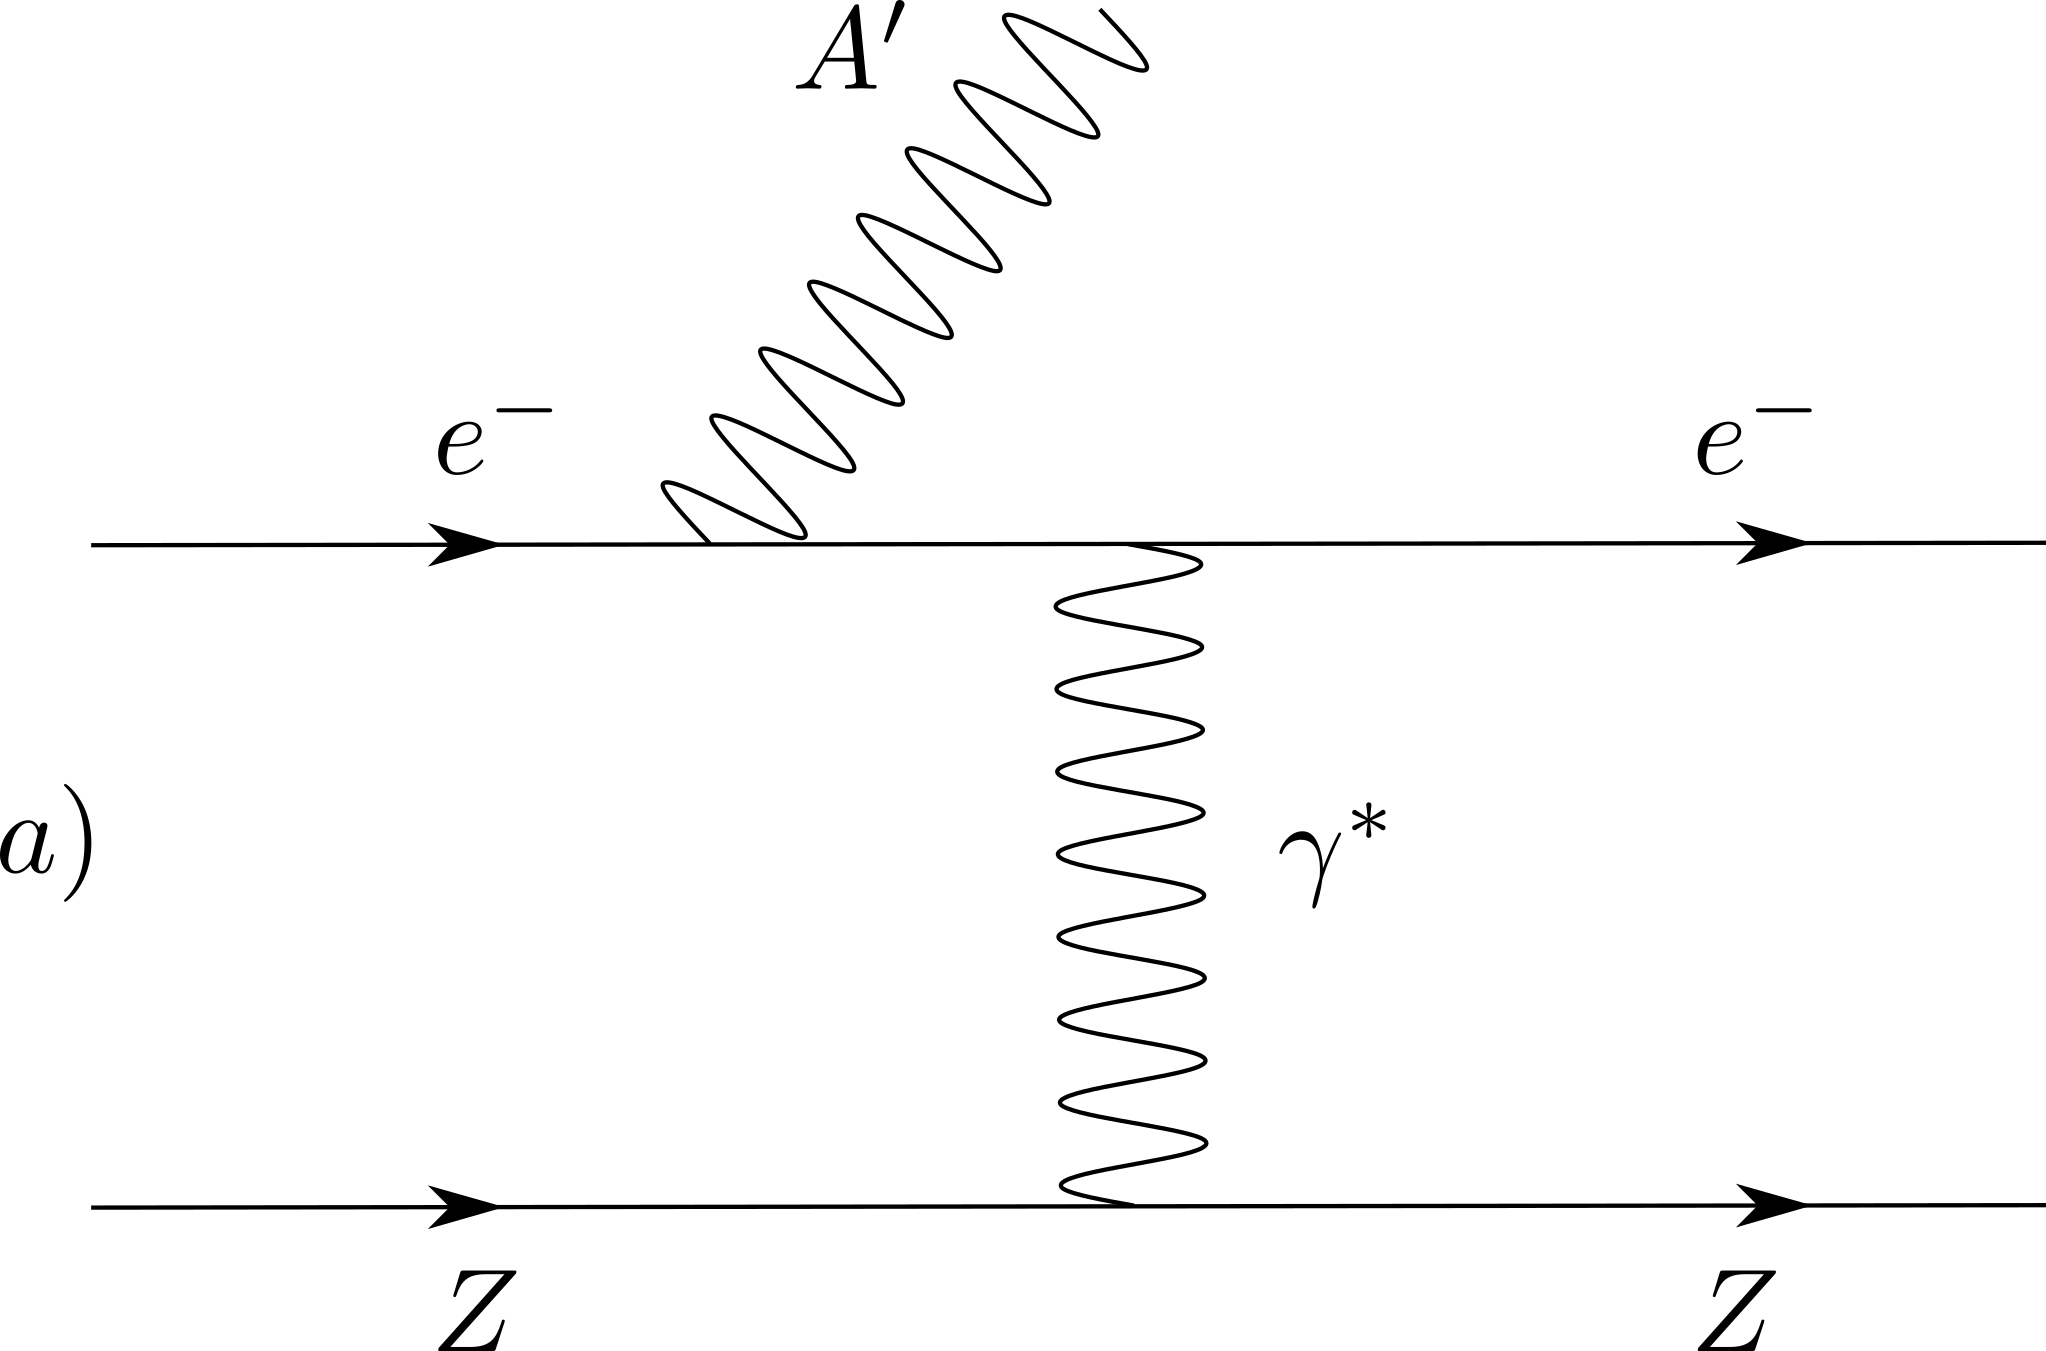
\includegraphics[width=.45\textwidth]{\pdirtwo/DarkBremstrahlung.png}
  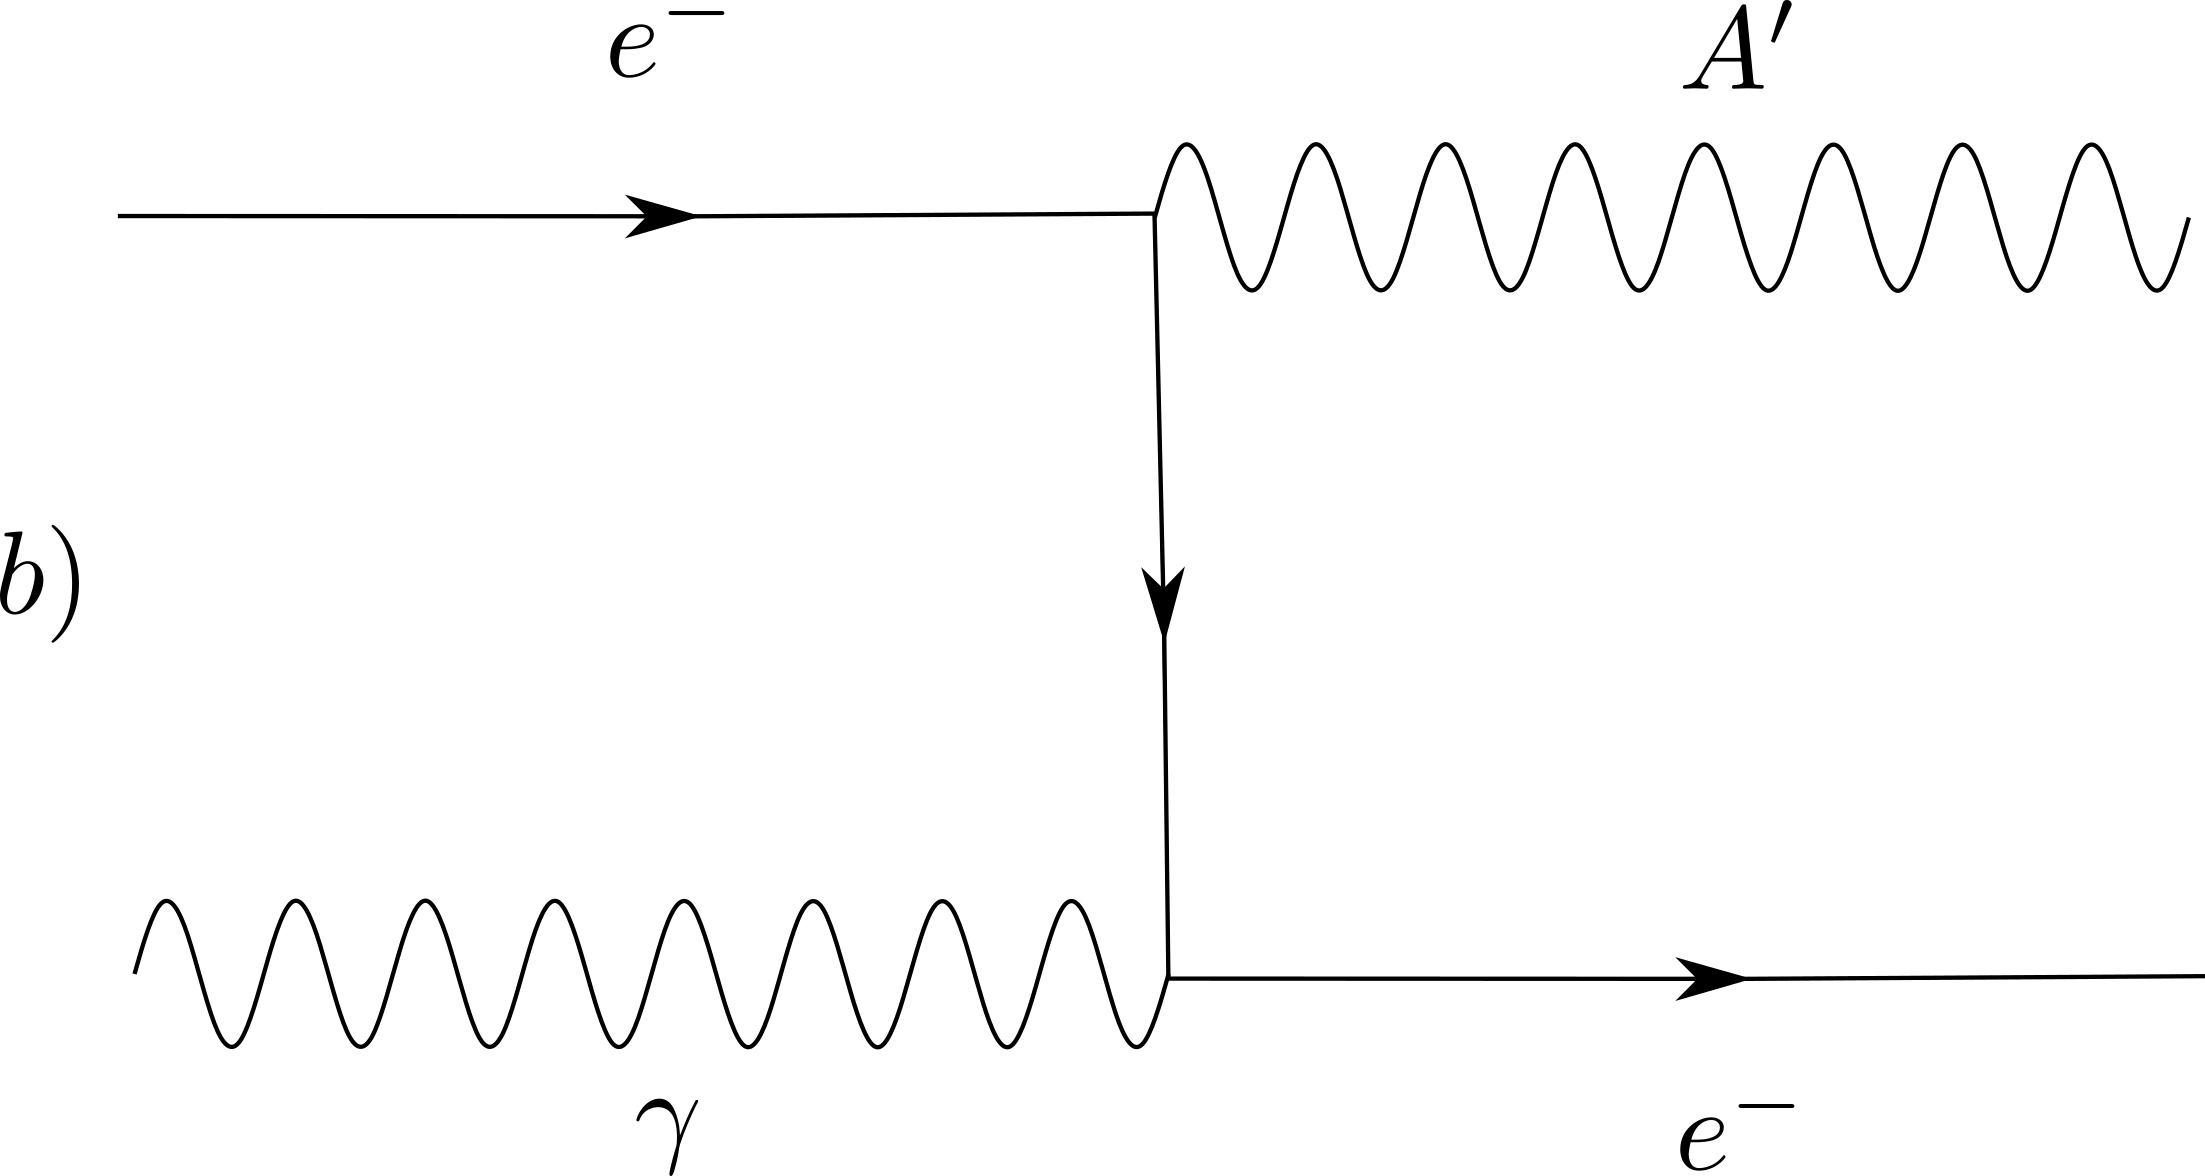
\includegraphics[width=.45\textwidth]{\pdirtwo/DarkCompton.png}
  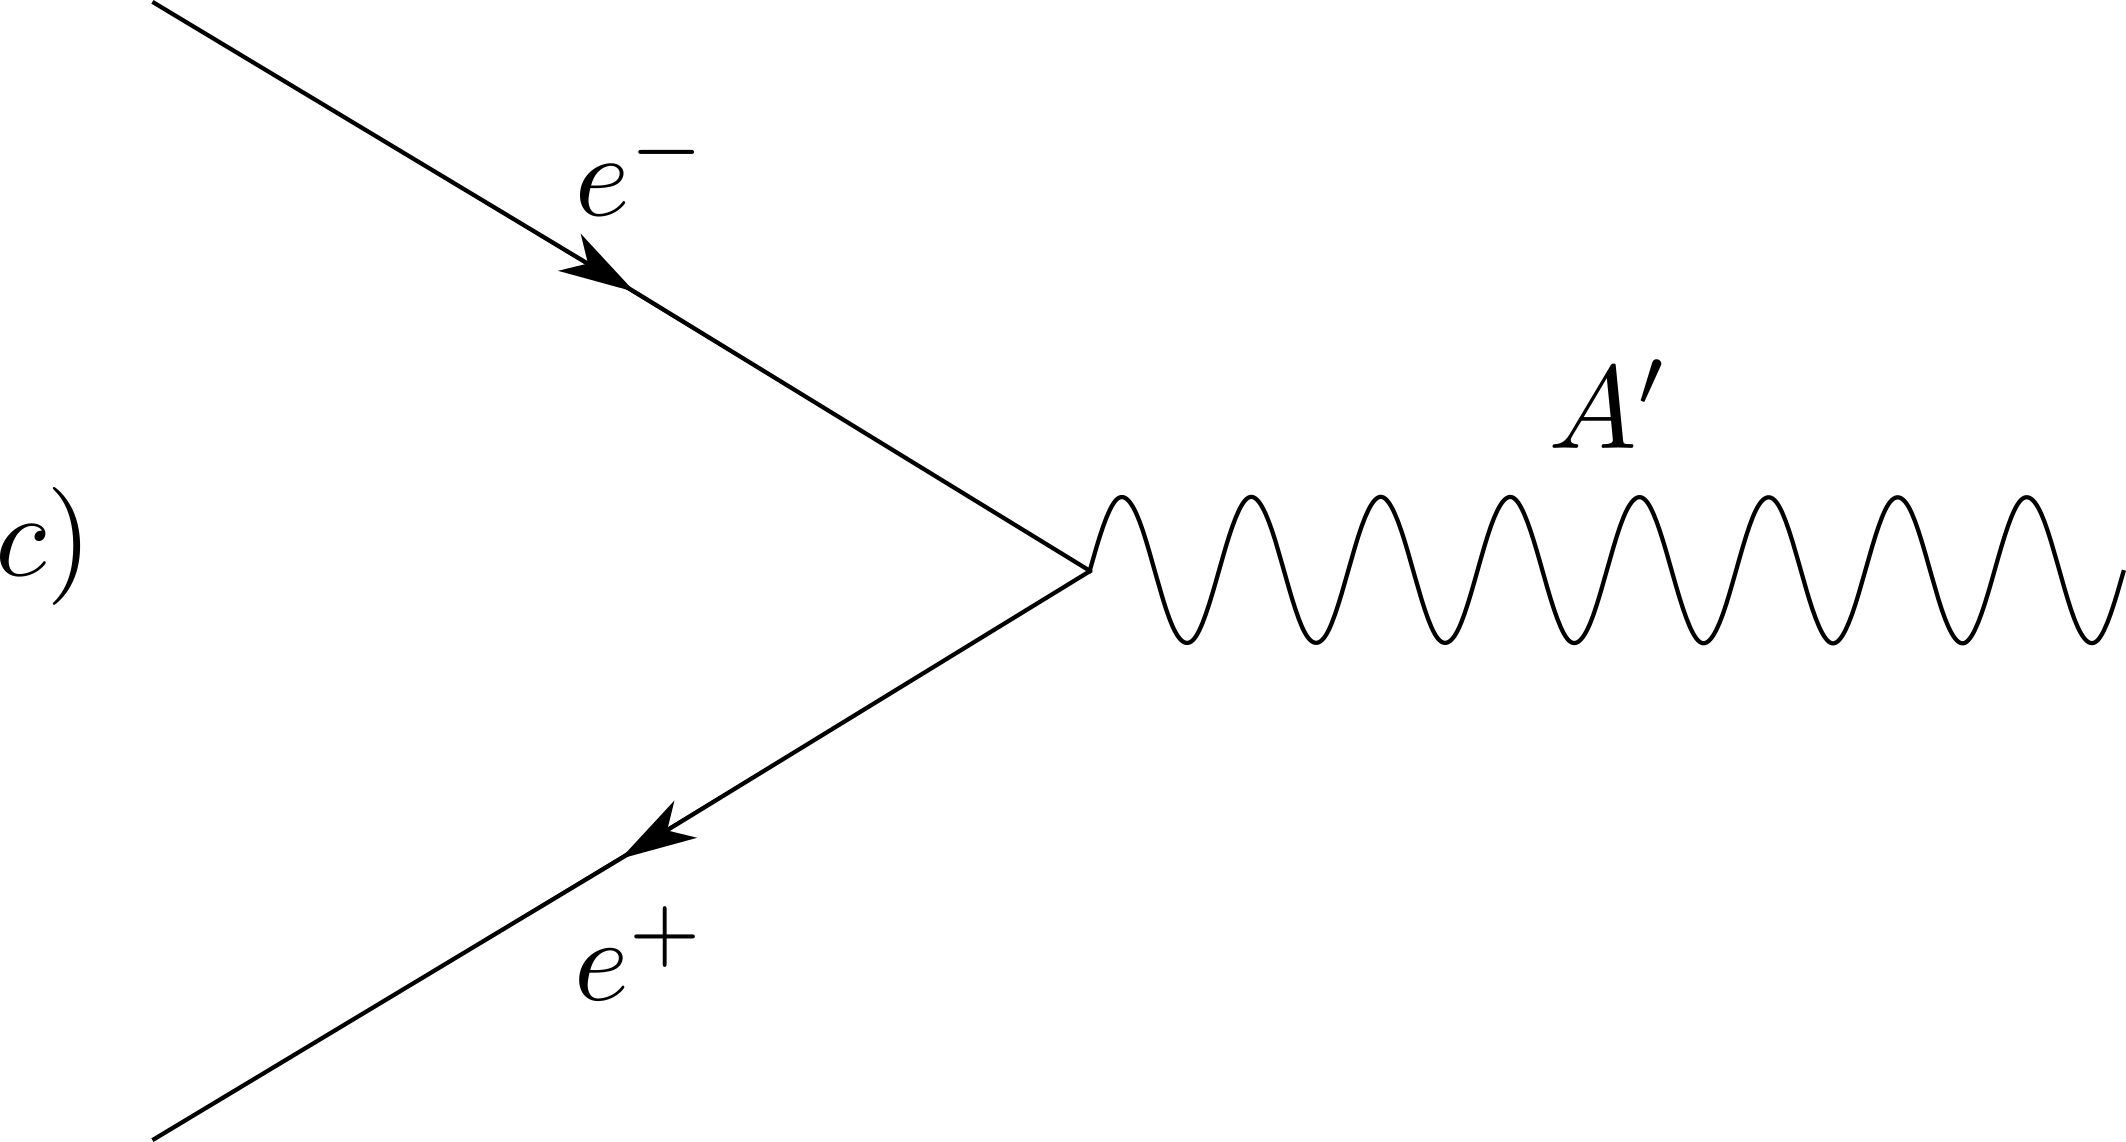
\includegraphics[width=.45\textwidth]{\pdirtwo/DarkResonance.png}
  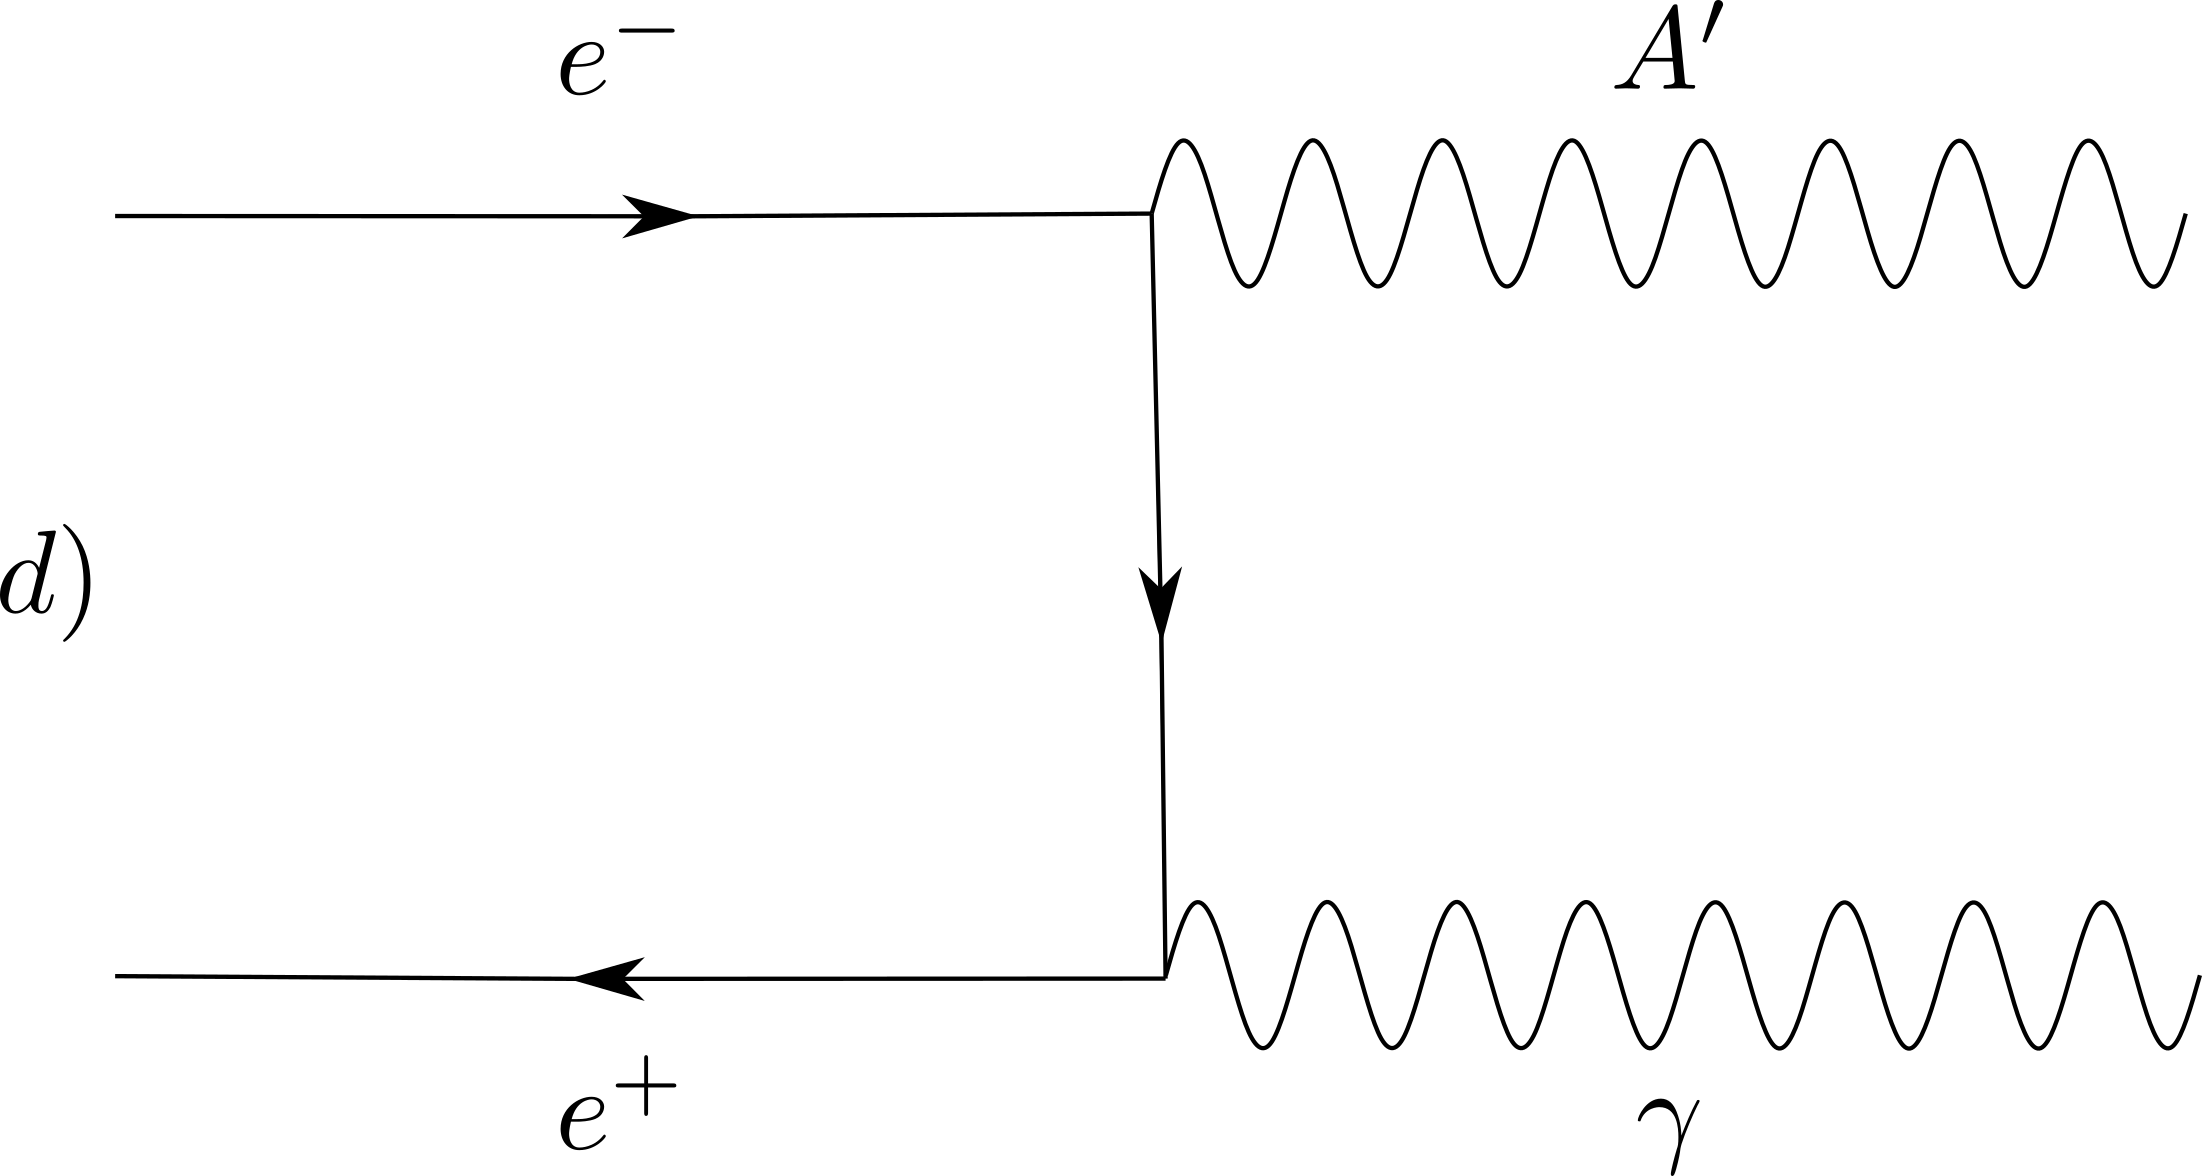
\includegraphics[width=.45\textwidth]{\pdirtwo/DarkAresonance.png}
  \caption{Possible production mechanism for $\DM$: Dark Bremsstrahlung a), Dark Compton b), resonance production c) and A-resonant production d).}
  \label{fig:dm-production-mechanism}
\end{figure}

One has to be careful and consider the list above a simple guideline that is in no way exhaustive. Other channels might be possible with minimal extension of the model, or one could find a significant yield of production not only in the scattering of an electron but also in more exotic physic. An example would be using the electromagnetic portion of large hadron shower to compute the yield of $\DM$. This was for example claimed to be a useful method to search for low mass $\DM$ in \cite{Celentano:2020vtu}.

A careful reader might object that the particles needed for each production channel are different. Indeed while a nuclei Z is always present in matter, the presence of a $\gamma$ or a $e^+$ might not be as straightforward. We remind here however, that in an electromagnetic shower originated by an high energetic lepton all three particles will be produced in large quantity due to the subsequent process of pair-production and Bremsstrahlung that are the most relevant for high energetic $\gamma$ and high energetic $\ee$ respectively. A complete review of electromagnetic and hadronic shower can be found here \cite{Bichsel:2002cf} for the interested. Indeed the production mechanism will be more relevant later when the analysis is performed, in normal circumstances when an high energetic particle hit a thick target all of the mentioned mechanism will be relevant to some degree. In our case, the Dark Bremsstrahlung $\darkbrem$ is used "Golden Channel" for the production. The reason is that it is relatively easy to compute using analytical formulas in good approximation (see Appendix\ref{appendixA:sec:cross-section} for more details) and has a very good yield compared to the other channels. This is not to say that the other channel do not matter, but at this stage where the experiment is being design we will consider them as minor corrections to a production rate mostly dominated by the Dark Bremsstrahlung. To avoid confusion in the reader, we also admit here that an appropriate analysis might make such contribution very relevant. An example can be found in \cite{Marsicano_2018} where the non-resonant and resonant production are used to improve significantly the signal yield for specific mass range.

After the production mechanism is chosen, some first estimate on the signal yield can be performed. However successfully producing the particle is not by itself sufficient without a mechanism device to detect it. The question that becomes interesting here is: what happens to $\DM$ after it is produced inside a target? We remind the reader here that since a coupling between standard matter and dark matter was theorized in the $\umodel$ model, the $\DM$ will be able to decay in a $\ee$ pair (or in more massive leptons) provided that its mass is sufficiently large, but it could also decay in particles of the dark sector, the one called $\dmchi$ introduced in Sec.\ref{chapter1:sec:dm-u1model}. The exact branching ratio can be calculated to be:

\begin{equation}
  \label{chapter1:eq:dm-bratio}
  \Gamma(A'\rightarrow\dmchi) = \frac{\alpha_D}{3}m_{A'}(1 + \frac{2m^2_{\chi}}{M^2_{A'}})\sqrt{1 - \frac{4m^2_{\chi}}{M^2_{A'}}}   
  \Gamma(A'\rightarrow\dmchi) = \frac{\alpha \epsilon^2}{3}m_{A'}(1 + \frac{2m^2_{e}}{M^2_{A'}}\sqrt{1 - \frac{4m^2_{e}}{M^2_{A'}}} 
\end{equation}

To simplify, we consider the two cases where the branching ratio is dominated by one single decay

\begin{itemize}
\item \textbf{Invisible decay:} If $\alpha_D / (\alpha \epsilon^2) \gg 1$ the A' will decay mainly in $\dmchi$. This decay is called invisible, as the decay products interact very weakly with standard matter
\item \textbf{Visible decay:} If $\alpha_D / (\alpha \epsilon^2) \ll 1$ the A' will decay mainly in $\ee$. This decay is called visible, as the decay products can be easily detected since they posses an electromagnetic charge. 
\end{itemize}

As always we need to admit that the physics always offer a plethora of possibilities that are not always easy to summarize in a thesis. There is no meaningful constraint that prevent both branching ratio to be on a similar footing. Likewise models with more complicate decay are possible. An example is the one illustrated in \cite{Mohlabeng_2019}, where the decay chain $\dmsemivis$ dominates. It is of course possible to adjust the setup to be more sensitive to specific model that turn out to be interesting, but in the interest of time we will focus on the two channel explained above that outside of being interesting are the main interest of the NA64 experiment.

The technique used in NA64 to detect this two channels will be explored in Sec.\ref{chapter2:sec:experimental-technique}. After that, the two setup designed for each of the specific two cases will be described in Sec.\ref{chapter2:sec:experimental-setup}. Finally, a detailed description of each detectors involved and their purpose will be outlined in Sec.\ref{chapter2:sec:detectors}.


\section{Experimental Technique}
\label{chapter2:sec:experimental-technique}

The detection of the $\DM$ needs to follow different strategies depending on what decay channel it is favored by it. If $\DM$ decays mainly into $\dmchi$, one could try to detect one of the two particles using a very thick detector. Indeed this is possible since by definition in the $\umodel$ a portal exist that connects dark matter to the classical one. However such an experiment will have a very limited reach, not only a factor $\alpha \epsilon^2$ needs to be "paid" to produced $\DM$ but an additional $\alpha \epsilon^2$ is also needed in order to detect its decay product. It is clear that especially for low coupling $\epsilon$ the probability to detect a single $\DM$ becomes  vanishingly  small. The second possibility is to make the disappearance of energy the signal of the experiment, i.e. assuming that the energy of $\DM$ is completely lost in the event. Such an experiment needs only to produce $\DM$ and does not need to worry about what happen to the particle after. To design a setup able to characterize this type of signature properly, we need to worry about the following items:

\begin{itemize}
\item The initial momentum of the particle needs to be well known
\item The setup needs to be completely hermetic, i.e. no energy can escape detection without using the channel under study
\item The initial particle ID needs to be well known
\end{itemize}

While the two first item are fairly trivial, one could wonder why the last one is necessary. Clearly if we need to apply any kind of statistical analysis to our data one has to know the total number of the electron that impact our target, the so called Electron On Target (EOT), so in this sense to understand the sensitivity of the experiment suck knowledge is necessary. On top of this however, the particle ID is necessary also to distinguish events that are in our signal box even if no $\DM$ is being produced. A precise background discussion is left for Chapter \ref{chapter3}, here we just provide the example of the decay chain $K^- \to e^- \nu_e$ \cite{review-particle-physics}: if a $K^-$ hits the target without being properly distinguished, it is possible for it to leave an electromagnetic signature and at the same time transport some energy out of the setup via $\nu_e$. This is exactly the signature we would expect for $\DM$! Hence the necessity of some system able to distinguish between particle of different species.

What about the visible mode? If we assume the decay $\aee$ is prominent, it is clear that missing energy can no longer be considered a signature. One should search for a $\ee$ pair in the final state, these particles are however very common in particle physics experiment, so one has to think how to characterize the event more. The property that mostly characterize dark matter is its inability to interact with ordinary matter, and hence travel freely inside very dense material. Since $\DM$ travels for a finite distance before decaying, if the target is thick enough, the only way to see an $\ee$ emerging from the target will be that a $\DM$ is being produced. A simple $e^-$ will be stopped by the thick target and nothing will emerge on the other side of the wall. If on the other hand we measure an high-energetic $\ee$ pair emerging on the other side of the wall and the energy of this pair matches exactly the one that is missing from the target, we conclude that the energy was transported outside the volume using a neutral boson. Assuming that no such channel exist in the standard model (which is to be demonstrated with a detailed background study) we can claim the observation of an event compatible with our hypothesis! Noticed in this case as well the three properties listed above are necessary, indeed one needs to know with good precision the initial momentum of the particle hitting the target and be sure that the particle is an electron. In this case however, the signal is not missing energy but instead energy conservation between a detector placed upstream and the one placed downstream. If we assume the energy of the primary electron to be $E_0$ and we plot the energy recorded in the two calorimeter, we can conceptualize the difference between the two signature in Fig.\ref{fig:two-signature}. As one can see, we are assuming here that the first calorimeter is able to stop the incoming particle with 100\% efficiency, and that therefore the only way to reach the downstream calorimeter is via the production of dark matter.

\subsection{invisible decay mode}
\label{chapter2:sec:experimental-technique-invis}

\subsection{visible decay mode}
\label{chapter2:sec:experimental-technique-vis}

\section{Experimental setup}
\label{chapter2:sec:experimental-setup}

\subsection{The invisible mode setup}
\label{chapter2:sec:invismode}

\subsection{The visible mode setup}
\label{chapter2:sec:vismode}

The method of the search for $\aee$ (or $\xdecay$) decays is detailed in \cite{Gninenko:2013rka, Andreas:2013lya, gkkk1, DMsimulation}. Here, we review it briefly. The $\DM$ is produced via scattering of 150 GeV electrons off nuclei of an active target-dump. The $\DM$ production is followed by its decay into $\ee$ pairs:
\begin{equation}
e^- + Z \to e^- + Z + \DM   ;~ \DM\to \ee \,.
\label{ea}
\end{equation}


\begin{figure}[tb]
\centering
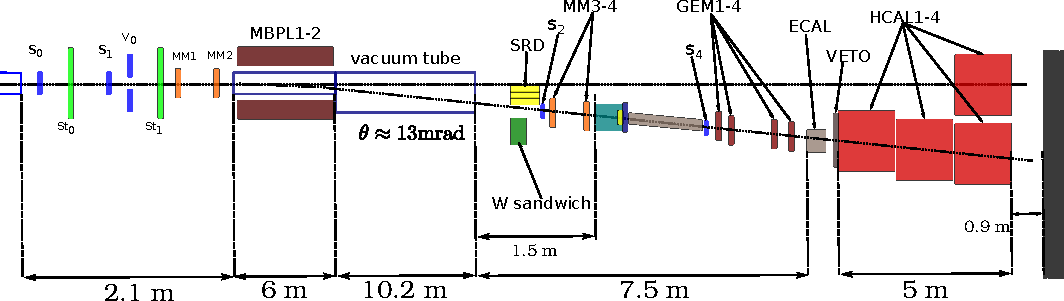
\includegraphics[width=1.\textwidth]{\pdirtwo/NA64_setup_2018_visible.pdf}
\caption[NA64 visible mode setup 2018]{The setup to search for $\DM$$\to \ee$  decays of the bremsstrahlung $\DM$ produced in the reaction
$eZ \to eZ+\DM $ of the 150 GeV electrons incident on the active WCAL target.}
\label{fig:setup-2018}
\end{figure}

The NA64 experiment searched for these decays using the H4 beam line of the CERN Super Proton Synchrotron (SPS) delivering about  $\simeq 5\times 10^6~e^-$ every 4.8 seconds. The setup used for this search is shown in Fig.\ref{fig:setup-2018}. A spectrometer made of a bending magnet combined with trackers measures the particle momentum. The magnet allows as well a very efficient electron identification (ID) using a Synchrotron Radiation Detector(SRD). Hadrons are additionally suppressed using a high efficiency VETO and a set of 3 hadronic calorimeter modules (HCAL) placed at the end of the setup. To measure the energy of the $\ee$ in signal events a highly-segmented electromagnetic-calorimeter (ECAL) is placed downstream of the decay volume. The signal region is defined by the sum of energy deposited in both calorimeters being compatible to the original beam energy. Additionally, the energy deposited in the last layer of the WCAL (W$_2$) is required to be lower than one Minimum Ionizing Particle (MIP) to suppress punch-through from the electromagnetic shower.

The allowed coupling $\epsilon$ for the $\DM$ can be as high as $1.4 \times 10^{-3}$, resulting in a very short decay length of few mm. Therefore, to boost the signal yield one should reduce the length of the active target to enhance the number of decays outside the dump. Additionally, for an unambiguous signature of the $\DM$ production it is crucial to reconstruct the invariant mass of the particle's decay. The small decay angle of $\DM$ ($\sim$0.3 mrad) makes this task particularly challenging. Therefore, a long decay volume must be used to resolve the two tracks.

\section{Detectors}
\label{chapter2:sec:detectors}

\subsection{The Trigger system}
\label{chapter2:sec:detectors-trigger}

\subsection{The Electromagnetic Calorimeter (ECAL)}
\label{chapter2:sec:detectors-ecal}

\subsection{The Hadronic Calorimeter (HCAL)}
\label{chapter2:sec:detectors-hcal}

\subsection{The Synchrotron radiation detector (SRD)}
\label{chapter2:sec:detectors-srd}

\subsection{The Veto system}
\label{chapter2:sec:detectors-veto}

\subsection{The Tracking system}
\label{chapter2:sec:detectors-tracking}

\subsection{The data Acquisition system (DAQ)}
\label{chapter2:sec:daq}

%%% Local Variables:
%%% mode: latex
%%% TeX-master: t
%%% End:
